\documentclass[dvipdfmx,11pt,a4paper]{jsbook}
\usepackage{package}
%\usepackage{a4wide}
\usepackage[dvipdfmx]{hyperref}
\usepackage{pxjahyper}


%\title{}
%\author{}
%\date{\today}
\begin{document}
%\maketitle

%\tableofcontents

\makeatletter
\@addtoreset{equation}{section}
\def\theequation{\thesection.\arabic{equation}}
\makeatother

\addtolength{\fullwidth}{-26truemm} %全体の幅(ヘッダ部の幅)を既定値から26mm小さくする
\setlength{\textwidth}{\fullwidth}  %本文の幅(textwidth)を全体の幅(=ヘッダ部の幅)にそろえる
\setlength{\evensidemargin}{10truemm}   %偶数ページの左余白を10mm(+1インチ)にする
\setlength{\oddsidemargin}{10truemm}    %奇数ページの左余白を10mm(+1インチ)にする

\chapter{CLASSICAL SOLITONS AND SOLITARY WAVES}
\begin{itembox}[l]{目的}
    非線形方程式の古典解のうち,ミンコフスキー計量やユークリッド方程式における場の方程式に対応するものがいくつかあり,そういった古典解から相対論的量子場の理論の情報を得る.
\end{itembox}

\section{Introduction}

本ゼミにおいてのメインテーマとなるソリトンとインスタントンであるが,どちらも簡単にいえば形状を保ったまま進行し互いに衝突・追突しても崩れないような局在化(localized)した波の事である.そもそもソリトンの英語スペルはsolitonであり,これはsolitary(孤立した)+on(粒子につける接尾辞(Fermi{\bf on}, Bos{\bf on}, Glu{\bf on}, Phot{\bf on} \dots))から来ている.すなわち孤立した波の塊でありながら歪むことなく安定に一様な速度で進行する波であり,粒子的に振る舞うような物理的対象を指す.ここで,なぜ局在化した波が粒子としてみなせるかということについては場の理論において場が作る波をエネルギーのたまり場のようなものであると捉えると,ポツンと局在化したエネルギーが非離散的(連続的)に形を崩さずに移動していればまるで粒子が移動していると拡大解釈できることから理解できる.

このようなソリトンは様々な応用が効く.本来素粒子は量子論で語られるべきものであるが,相対論的な場の理論から素粒子もlocalizeされたエネルギーパケットをもっていることがわかっており,古典場の理論からスタートするソリトンを用いてその振る舞いを説明することができ,ソリトンが古典論と量子論をつなげる可能性を持ち合わせていることを意味する.他にもソリトンには原子核,陽子中性子の模型や宇宙論のテクスチャ,物性の磁気スカーミオンなど素粒子原子核から物性,宇宙まで様々な分野において重要な役割を果たす.

\begin{figure}[H]
    \centering
    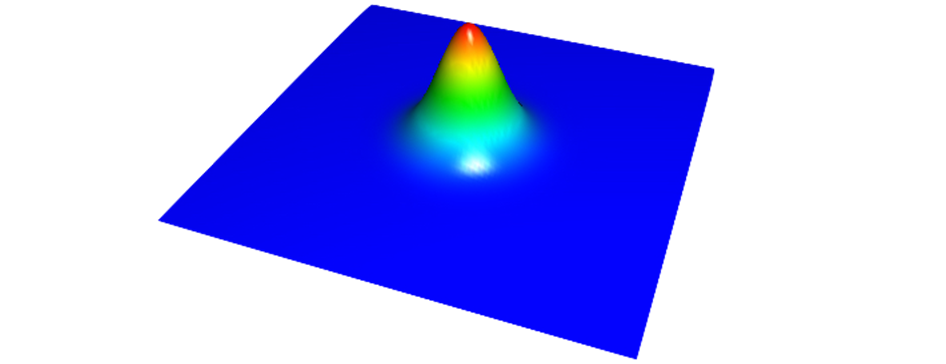
\includegraphics[width=8cm]{figure/soliton.png}
    \caption{ソリトン}
    \label{soliton}
\end{figure}
本章におけるメインテーマはsin-Gordons solitonやkinkの$\phi^4$理論や'tHooft-Polyakov monopoleやインスタントンなどの例を用いながらソリトン(Solitons)と孤立波(Solitary waves)の区別をつけるということである.

また,以下にこれから使う記法についてまとめておく.
\begin{screen}
    \begin{itemize}
        \item 空間と時空の座標系はベクトル$x^{\mu}(\mu=0, 1, 2, 3, ; x^{0}\equiv ct, x^{1}=x, x^{2}=y, x^{3}=z)$で与えられる.
        \item 上付きまたは下付きの添字はミンコフスキー計量テンソル$g_{\mu \nu}=g^{\mu \nu}$;
              \begin{align*}
                  g_{\mu \nu}=
                  \left(\begin{array}{cccc}
                          1 & 0  & 0  & 0  \\
                          0 & -1 & 0  & 0  \\
                          0 & 0  & -1 & 0  \\
                          0 & 0  & 0  & -1
                      \end{array}\right)
              \end{align*}
              で書かれる.(Mostly minus)
        \item 同じ添字がついてるものについては足し上げる.(縮約記法)
        \item $\partial_{\mu}$は時間や空間での微分$\frac{\partial}{\partial_{\mu}}$を表す.
        \item 簡単のために本セクションに限っては1つの時間座標と1つの空間座標の(1+1)次元,つまり$\mu=0,1$とする.
    \end{itemize}
\end{screen}

\section{Solitary waves and solitons}
先に述べたようにSolitonとSolitary waveは非線形の波動方程式においてどちらも局在化した特別な特徴をもつ解でありその区別はどのようにできるかを学ぶ.

まず,よくある最もシンプルな線形かつ非分散的である波動方程式
\begin{align}
    \Box\phi & =\partial^{\mu}\partial_{\mu}\phi\nonumber                                                                          \\
             & =\left(\dfrac{1}{c^2}\dfrac{\partial^2}{\partial t^2}-\dfrac{\partial^2}{\partial x^2}\right)\phi(x,t)=0\label{2.1}
\end{align}
を考える.この解は以下のような2つの特徴をもつ.
\begin{description}
    \item[(i)] 解である$f(x\pm ct)$は全領域で一意に定まり,微分が定義され,連続である(well-behaved function).また,$\omega=kc$とすれば$\cos(kx\pm \omega t)$と$\sin(kx\pm \omega t)$の平面波はどちらも式(\ref{2.1})の1つの解となっておりフーリエ変換で重ね合わせれば
          \begin{align}
              f(x-c t)=\int \mathrm{d} k\left[a_{1}(k) \cos (k x-\omega t)+a_{2}(k) \sin (k x-\omega t)\right]
          \end{align}
          とかける.そして仮に局在化した解$f(x-ct)$をもってきた場合,その波のパケットは一定速度$\pm c$で歪みや形の崩れなく進む.
    \item[(ii)] 波動方程式が線形であるが故に解として波のパケット$f_1(x-ct)$と$f_2(x+ct)$が与えられれば,それらの線形結合である
          \begin{align}
              f_3(x,t)=f_1(x-ct)+f_2(x+ct)
          \end{align}
          もまた解となる.

          そして$t\rightarrow-\infty$で$f(x,t)$は2つのパケットはそれぞれ別の方向に向かって二分され,その後時間をかけて互いに歪まずに接近し衝突する.そして衝突後も形を崩さず$t\rightarrow\infty$に向かって同じ2つのパケットが一定の速度で移動していく.
\end{description}
つまりこれらを簡単にまとめれば式(\ref{2.1})の解は以下の性質を持つ.
\begin{screen}
    \begin{description}
        \item[(i)] 1つのパケットが歪まず,形を維持したまま一定速度で移動する.
        \item[(ii)] いくつかのパケットが互いに衝突したとしてもその進行速度と形が維持される.
    \end{description}
\end{screen}
しかしながら大半の波動方程式は非線形校を含んでいたり,分散的であったりと複雑で全ての波動方程式が性質(i),(ii)を満たしているとは限らない.

そのうちの一つが式(\ref{2.1})に$m^2c^2$の項を加えたKlein-Gordon方程式
\begin{align}
    \left(\square+m^{2} c^{2}\right) \phi(x, t) & \equiv\left(\frac{1}{c^{2}} \frac{\partial^{2}}{\partial t^{2}}-\frac{\partial^{2}}{\partial x^{2}}+m^{2} c^{2}\right) \phi(x, t) \\
                                                & =0
\end{align}
がある.これは明らかに先と同様に線形でありながら$\cos(kx\pm \omega t)$と$\sin(kx\pm \omega t)$の平面波解をもつ.しかし今回の場合は$\omega^2=k^2c^2+m^2c^4$であり

\end{document}
